\documentclass[11pt]{article}

\usepackage{a4wide}
\usepackage{mathptm}
\usepackage{xspace}
\usepackage{amsmath}
\usepackage{graphicx}
\usepackage{algorithm}
\usepackage{algpseudocode}
\usepackage{tikz}
\usepackage{tkz-graph}
\usetikzlibrary{shapes.misc, positioning}
\usepackage{listings}
\usepackage{color}

\definecolor{dkgreen}{rgb}{0,0.6,0}
\definecolor{gray}{rgb}{0.5,0.5,0.5}
\definecolor{mauve}{rgb}{0.58,0,0.82}

\lstset{frame=tb,
  language=Java,
  aboveskip=3mm,
  belowskip=3mm,
  showstringspaces=false,
  columns=flexible,
  basicstyle={\small\ttfamily},
  numbers=left,
  numberstyle=\tiny\color{gray},
  keywordstyle=\color{blue},
  commentstyle=\color{dkgreen},
  stringstyle=\color{mauve},
  breaklines=true,
  breakatwhitespace=true,
  tabsize=3
}
\begin{document}

\title{Framework Face Off}

\author{Jonatan Valen, Daniel Nyvoll & Vegard Vasset}

\maketitle

\begin{abstract}

  10-15 lines with the software technology and the highlights from the
  project that has been undertaken.

\end{abstract}

%\input{commands}

\section{Introduction}

In the dynamic world of web development, choosing the right front-end framework is crucial yet challenging, especially for novices in the field. With the rapid evolution of the digital landscape, developers, particularly those inexperienced with front-end frameworks, face a challenging decision. In our study, which we conducted without any prior knowledge of front-end frameworks, we hypothesize that a thorough comparative analysis of prominent frameworks like React, Svelte, and Vue can clarify their strengths and weaknesses. This approach aims to aid beginners in making an informed decision about which framework to learn and use.
The decision of selecting a front-end framework is critical. It profoundly influences the development process, application performance, and end-user satisfaction. As the web becomes increasingly integral to our daily lives, ensuring the optimal performance and usability of web applications is not just a technical concern but a necessity for enhancing digital experiences globally.

To address this, our project aims to conduct a comprehensive comparative study of React, Svelte, and Vue. We intend to evaluate these frameworks across crucial parameters like documentation, runtime performance, code quality, and cross-browser compatibility. Our approach involves developing a web application using each framework, adhering to test-driven development principles to ensure consistency and fairness. This methodical evaluation will not only compare these frameworks but also provide insights into their suitability for various development scenarios. 

To expand on this, our project will also place significant emphasis on the subjective experience of the development process. As newcomers to the realm of front-end frameworks, we will document our personal journey with React, Svelte, and Vue. By reflecting on the intuitiveness of the frameworks, the clarity of documentation, and the ease of overcoming challenges, we aim to provide a unique perspective on the learning curve and developer ergonomics of each framework. This personal narrative will complement our objective metrics, offering a comprehensive view of the frameworks from the standpoint of novice developers. This experiential component could be invaluable for beginners who are evaluating these tools for their own use.


\subsection*{Background}

Representing the popularity trends of various web development frameworks over a period from 2016 to 2019

React, known for its robust ecosystem and backing by Facebook, has consistently held a significant share of popularity, while Vue.js has emerged as a strong contender with its approachable learning curve and incremental adoptability. Meanwhile, Svelte, the newest among them, presents an innovative approach by shifting work to compile time, leading to faster runtime performances.

To ensure a consistent standard of functionality across the web pages developed using each framework, Test-Driven Development (TDD) was employed as an aspect of our comparative analysis. This approach guaranteed that, although different frameworks were used, each implementation adhered to the same functional specifications. By integrating TDD into our workflow, we were able to provide a more objective measure of each framework's capabilities, taking into account not only the end product but also the development process itself.

In our analysis of front-end frameworks, we selected a weather application as our use case, primarily because it allows for practical experimentation with public APIs. This choice provided a tangible means to assess and compare the capabilities of various frameworks in handling real-time data, user interface dynamics, and responsiveness. The weather application scenario was particularly suited for this comparison as it involved fetching and displaying data from external sources, a common requirement in modern web development. This setup enabled us to evaluate how different the frameworks React, Svelte and Vue.js manage data binding, state management, and overall performance. Additionally, the integration with public APIs served as an excellent benchmark for understanding the ease of use, flexibility, and scalability offered by each framework, making our comparison comprehensive and relevant to current industry trends.

Central to our approach was the utilization of client-side operations, primarily fetching data from various APIs. The decision to not set up a dedicated backend allowed us to concentrate on the frontend functionalities, exploring how each framework handles tasks like API calls, data processing, and DOM manipulation. By simulating real-world scenarios where frontend applications interact with existing APIs, we were able to assess the efficiency, ease of integration, and responsiveness of each framework in handling client-side operations.


\subsection*{Implementation}

\subsubsection*{Test Driven Development}

3.1 TDD

The implementation of Test-Driven Development (TDD) in our project commenced with the creation of unit tests before the actual coding of the application. We used testing frameworks like Jest and Vitest to write tests for core functionalities. For instance, we wrote tests to ensure the correct conversion of location names to geographic coordinates, a fundamental feature for our weather application. These tests validated the functionality of our geocoding utility and weather API services, ensuring that, for example, inputting 'New York' would correctly yield the expected latitude and longitude. Our project's testing phase was designed to maintain identical logic across Svelte, React, and Vue, allowing us to compare each developer's experience in achieving the required test outcomes. The journey to passing the tests provided insights into the user-friendliness of each framework, the quality and accessibility of their documentation, the richness of resources available, and the level of community support. These factors collectively offered a measure of each framework's approachability and practicality from a developer's perspective, influencing our overall evaluation of the tools.





\subsubsection*{React Implementation}

3.1 React Implementation

The React application is constructed with a focus on modular design, leveraging the power of React's component-based architecture. Each component is tailored to fulfill specific functionalities, contributing to a cohesive user experience. The application effectively utilizes state management through React hooks and engages with external APIs, ensuring dynamic content delivery and interaction.

Routing and Application Structure




The code snippet above is part of the App.js file. It illustrates the App component, which is responsible for the applications routing structure. It utilizes the Router component to define the applications navigation. Inside the Router, various Route components map URL paths to corresponding React components. For instance, the path /weather is associated with the WeatherApp component, while /active-transportation is linked to the Active-transportation component. There are also placeholder routes, which serve as temporary stubs for future implementation, denoted by the PlaceHolderApp component.

React root rendering: 


This code snippet is from the index.js file. It showcases the root rendering process of the React application. It uses React.StrictMode, which is a tool for highlighting potential problems in an application. I do not render any visible UI, but activates additional checks and warnings for its descendants. It is then passed to REACTDOM.createRoot, signifying the entry point of the application. This is where React elements are rendered into the DOM, with the root DOM node being provided by document.getElementByID(‘root’). This is what kickstarts the React application’s rendering process. 


Component Analysis: 

Reactive System and State Management:

The application's use of React hooks across several components like LocationMap.jsx, SearchBar.jsx, and Weather App.jsx. modern approach to state management. This setup ensures a responsive and user-friendly interface, capable of efficiently handling state changes and asynchronous operations.

For instance, in SearchBar.jsx React's useState  hook is employed to manage the state of the user's search input. This allows for an instantaneous and responsive feedback loop between the user input and the application's state. An example from the code illustrates this:


in the code snippet above we have the following key elements: 
useState hook. This is used to declare the state variable “searchTerm” and its updater function “setSearchTerm”. It is initialized with an empty string, and the state holds the current value of the search input. 
handleInputChange is an event handler function that updates the searchTerms state when with the value entered by the the user in the search input field
handleKeyPress is another event handler that listens for the “Enter” key press to trigger the search function passed as a prop. 

The component is designed to be reactive and responsive to user input, utilizing the useState hook for management and providing a clean and intuitive interface for users to perform search queries. 
Interaction with External APIs:


The application integrates with external APIs to enhance its feature set. In the code snippet above we see an example on how it is done in WeatherApp.jsx

An asynchronous function search is defined to handle retrieval of location coordinates and weather data. The application first uses Mapbox's Geocoding API to convert a location input into geographical coordinates. It constructs a request URL with the user's input from the cityInput field. Upon receiving the response, the application parses the JSON to extract latitude and longitude coordinates, which are then used to set the application's state with setLongitude and setLatitude.

With the coordinates obtained from Mapbox, the application proceeds to fetch weather data from the OpenWeatherMap API. It constructs a new request URL, including the latitude and longitude, and specifies the desired units as metric. The resulting weather data is obtained asynchronously, and the application updates the state with various weather details such as temperature, location name, humidity, wind speed, and a description of the current weather.

Once the data is retrieved and the state is updated, these values are used to update the UI, providing users with real-time weather information for the queried location. This is done using all the “set” functions. When these functions are called with new data retrieved from the API, they trigger a re-render of the component. 

\subsubsection*{Vue Implementation}
3.2 Vue Implementation: 



Vue Router:
Implementing routing functionality in Vue was remarkably straightforward and intuitive, primarily due to the seamless integration and alignment of Vue Router with the core Vue.js framework. Vue Router's declarative routing configuration, which leverages a simple and clear JavaScript object syntax, made it particularly easy to define and manage routes. This approach, combined with Vue's component-based architecture, allowed for an efficient and hassle-free setup of navigational structures within the application. Additionally, the comprehensive and well-organized documentation of Vue Router provided excellent guidance, further simplifying the implementation process.

Here is a code snippet of the implementation of Vue Router.

Component-based Development: 
The encapsulation of Vue components proved to be an intuitive and streamlined process, particularly advantageous for those new to frontend development. Components like SearchBar.vue or WeatherDisplay.vue function as standalone units, each with their dedicated HTML, CSS, and JavaScript. This encapsulation enables a focused approach on individual parts of the application, mitigating concerns about unintended interactions with other segments. The encapsulation was quickly recognized as beginner-friendly at the onset of development.

For example, WeatherDisplay.vue encapsulates the template, script, and style in a single file. The HTML structure, reactive data properties, methods, and component-specific styles are all consolidated, simplifying both development and troubleshooting.

The use of the 'scoped' attribute in the <style> tag is notably advantageous. It guarantees that the defined CSS styles are confined to the component, avoiding accidental style conflicts.

The facility to transfer data and methods via props and to issue events lends to the high reusability and maintainability of the components. Components like SearchBar.vue can be confidently utilized across various parts of the application, ensuring consistent and independent functionality.

The organization and modularity offered by Vue’s component system greatly reduce the complexity in developing an intricate web application, enabling a foundational understanding of each part of the application before their integration, which is substantially beneficial for learning frontend development effectively.

Reactive Data System:
The reactive data system in Vue.js offers a robust and streamlined mechanism for binding data to the user interface, facilitating the development of dynamic interfaces that update in real time. This system represents a paradigm shift away from the manual manipulation of the DOM, automating UI updates in response to state changes within the application.
In the context of the WeatherDisplay.vue component, the employment of Vue's reactive properties significantly simplifies the presentation of weather data. Through the declaration of a reactive data property within the component's data function, a direct linkage is established between the data and the template. Consequently, any modifications to the weather data are promptly and automatically mirrored in the UI, negating the need for extraneous code. This not only enhances efficiency but also underscores Vue's capability to streamline front-end development, particularly for those new to the framework.

Code snippets from WeatherDisplay.vue component, displaying current weather, demonstrating the use of reactive data binding: 

The {{ placeName }} interpolates the placeName data property into the heading. Whenever placeName changes, the content within the header tag will automatically update to reflect the new value.

The temperature, wind speed, and humidity are also dynamically rendered using data binding. 
For example, {{ weatherData.properties.timeseries[0].data.instant.air_temperature }} accesses the air_temperature property of the first item in the timeseries array from the weatherData object. This temperature value is displayed in the template.

Moreover, the v-if directive provides a declarative approach to controlling the visibility of DOM elements. It is used to conditionally render the container div for the weather data, based on the presence and truthiness of weatherData. This technique enhances the interface's reactivity and user experience by only presenting relevant information when data is available. The effectiveness of directives like v-if in managing the DOM underscores the strengths of Vue.js in creating interactive and reactive web applications.

Working with external APIs:
Engaging with external APIs within a Vue.js context proved to be an enriching educational experience, particularly in understanding and managing asynchronous operations. Initially, concepts such as asynchronous programming and API response handling appeared complex. However, the utilization of axios, a promise-based HTTP client, considerably simplified these tasks.

A practical application of this was demonstrated in the getCoordinatesFromName function, designed to transform a location name into geographic coordinates through the OpenStreetMap API. This function showcases the streamlined handling of HTTP requests facilitated by axios.

The use of async/await syntax in conjunction with axios greatly enhanced the readability and maintainability of the code. It allowed for writing asynchronous functions in a style reminiscent of synchronous code, thus simplifying the understanding and implementation. The getCoordinatesFromName function needed only the location name to perform its operation, handling the complexities of asynchronous requests and error management internally.

Following the acquisition of coordinates, the fetchWeatherData function was employed to retrieve weather data. 

These functionalities were integrated into a searchLocationByName function, providing a cohesive and user-friendly method for fetching and displaying weather data based on location names. This process underscored the importance of logical structuring in API calls and illustrated the effectiveness of JavaScript's advanced features in external API interactions. Such experiences highlighted the significance of adeptly handling asynchronous operations and leveraged the capabilities of modern JavaScript to enhance the application's functionality.

CSS and Responsive Design:
I discovered that implementing CSS and responsive design within my Vue components was both gratifying and educational. Initially, the thought of making my application look good on various devices seemed like a complex task. However, Vue's scoped styling feature was a great help. 

Challenges: 
Initial development stages revealed complexities in passing data between components lacking a direct parent-child relationship. It became evident that while props and events are suitable for communication within a direct lineage, they are insufficient for components situated far apart in the hierarchy. This prompted an exploration of the Vue.js ecosystem for solutions, leading to the discovery of state management patterns such as Vuex. 

\subsubsection*{Svelte Implementation}
3.3 Svelte implementation:

The Svelte application encapsulates a modular design ethos, mirroring the contemporary practices of component-based frameworks. In this Svelte-based project, each component is meticulously crafted to fulfill a discrete functional role, contributing to an integrated and seamless user experience. The application showcases a robust implementation of reactive state management, capitalizing on Svelte's innate reactivity and store capabilities.

The core of the application's routing is managed within the +page.svelte file, demonstrating Svelte's file-based routing mechanism. This approach is distinctly Svelte, where routes are implicitly defined through the file structure, streamlining the mapping of URL paths to Svelte components. The Menu.svelte component is responsible for navigating to different parts of the application, such as the weather view or the active transportation information section.

The application's reactive system is powered by Svelte's reactive stores, as seen in the store.js file. Svelte's reactivity is straightforward and less boilerplate-heavy compared to other frameworks, as any variable declared as writable in the store becomes reactive across the application. In Svelte, the $ symbol is used to denote a store value and to establish a reactive subscription to the store's changes. When the value of a store changes, any component that uses the $ syntax to refer to that store will automatically re-render to reflect the new value. The figure show the initialisation of the map by using the dollar sign:

Svelte's architecture is distinguished by its lifecycle hooks, which provide developers with fine-grained control over the behavior of components during their lifecycle events. Among these, onMount is a particularly crucial lifecycle hook used to run code when a component is first introduced into the DOM as seen in the figure.
The onMount function is typically employed for initialization tasks such as fetching data, setting up subscriptions, or directly interacting with the DOM, tasks that should only be executed once when the component is created.
Interacting with external APIs is a critical feature of the application. The code snippet provided indicates a function that interfaces with the Mapbox API, searching for locations based on user input. The seamless integration of API calls within Svelte components is indicative of the framework's promise to keep things simple and concise. The fetchData function shown in Figure??

Svelte's straightforward approach to incorporating asynchronous operations, showing how data fetched from an external weather API is utilized to update the reactive variables in the store, consequently refreshing the UI with new data.
The Svelte syntax allows for co-locating markup, script, and style, which is visible in the comprehensive <script> and <style>, making the codebase more maintainable and approachable.




\section{Evaluation}

In the final analysis of our front-end framework comparison for a weather application, several results stand out. React's build time is the longest at 9.7 seconds, which might be attributed to its comprehensive ecosystem that includes numerous libraries and plugins. While this can increase the initial load time, it offers a wealth of resources for API integration and the ability to efficiently handle dynamic data updates—a key aspect for real-time weather information.

Vue presents itself as a strong contender with the shortest build time of 4.9 seconds. This efficiency could reflect a more streamlined build process or a lighter framework footprint. Vue's performance advantage is evident during the initial development stages, contributing to rapid prototyping and early momentum in application development.

Svelte's build time stands at 6.44 seconds, positioning it between React and Vue. This intermediate value is reflective of Svelte's unique architectural approach, where much of the workload is shifted to compile time, resulting in optimized and concise final code. The Svelte store system, particularly its import/export functionality, plays a significant role in state management within the application, allowing for real-time updates across components without significant overhead.

Throughout the 16-week development period, the progress trajectory of each framework—Svelte, React, and Vue—revealed distinct patterns. Svelte's progression is characterized by a steady and consistent ascent, suggestive of an accessible learning curve and a development experience that grows more efficient with increased familiarity. In contrast, React's trajectory, while stable, was more gradual, reflecting its broader ecosystem and the complexity that comes with it. Vue showcased a swift climb, indicative of its initial ease of use and developer-friendly design, which may contribute to a quick uptake by new developers. However, this rapid progression could potentially level off as developers encounter the intricacies of advanced Vue concepts. Collectively, these patterns provide nuanced insights into the learning and development efficiencies of the three popular frameworks over a substantive period.

These measures of build time and application progress, coupled with qualitative feedback from developers, paint a comprehensive picture of each framework's strengths and weaknesses. They reveal not just the technical capabilities, but also the practical implications for developer productivity and application performance.

As emerging developers at the confluence of technological innovation and environmental responsibility, our assessment of carbon footprint and sustainability within the landscape of front-end development frameworks is more than academic—it is an ethical imperative. Recognizing that the digital solutions we craft today have a tangible impact on tomorrow's world, we diligently compared the sustainability profiles of Svelte, React, and Vue. Our criteria for evaluation were twofold: ease of use, which influences the speed and efficiency of development, and the carbon footprint, particularly influenced by daily build times. Svelte, with its lean build process and highly efficient runtime performance, emerged as the most sustainable framework in our study. Its build time, at 6.44 seconds, suggests a lower daily energy consumption, which, when scaled across the industry, could contribute significantly to energy conservation efforts. Coupled with its user-friendly approach, Svelte stands as a testament to our commitment to a sustainable future, blending ease of use with an environmentally conscious development process.

\subsection{Documentation and Learning Curve}

\begin{figure}[!htbp]
\centering
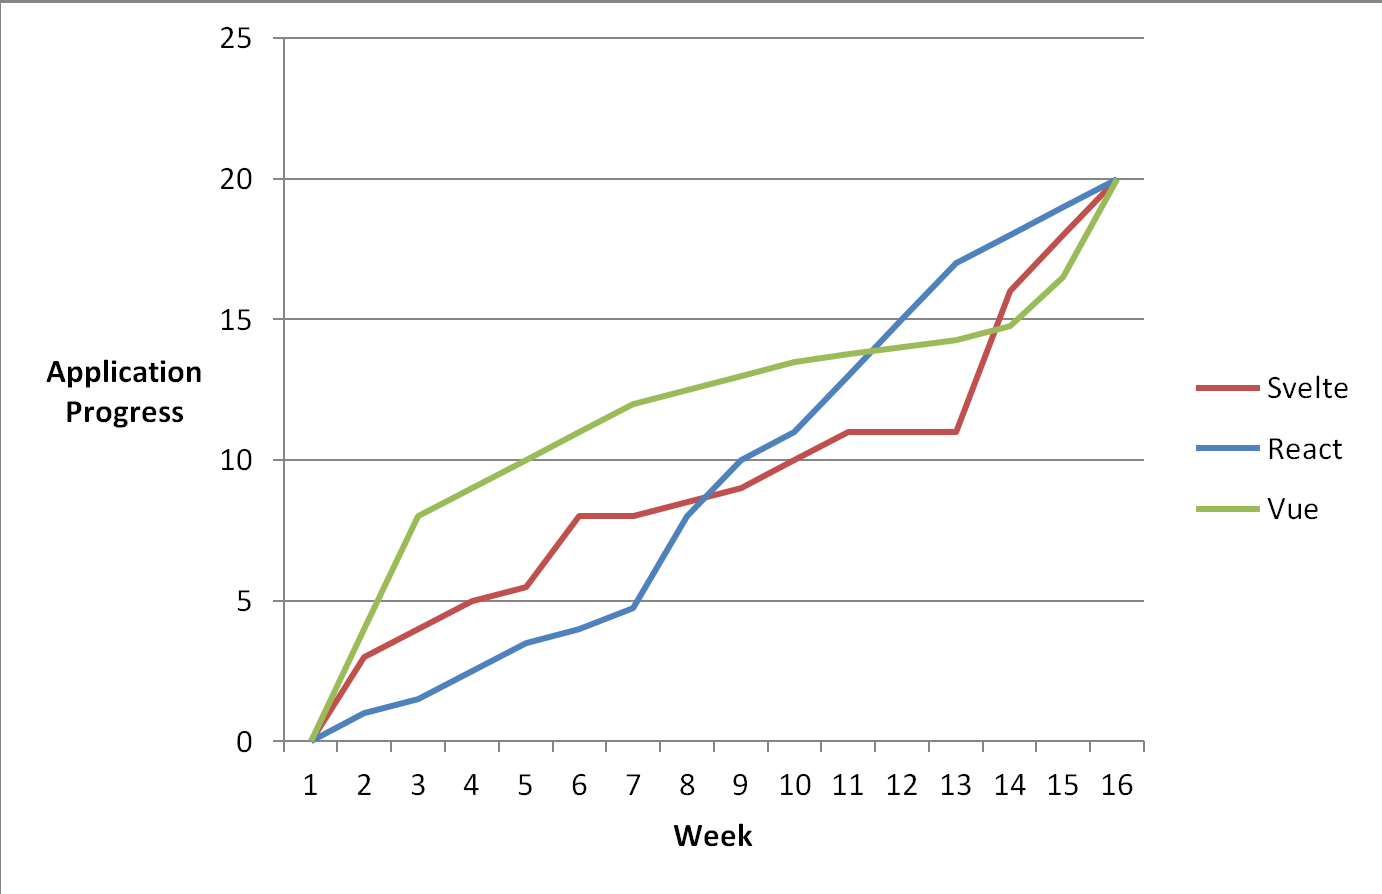
\includegraphics[width=\linewidth]{figs/progress.png}
\caption{progress}
\label{fig:progress}
\end{figure}

In our study, we found React's documentation to be exceptionally comprehensive. Covering everything from basic concepts to advanced topics like hooks and context, it served as a vital resource in our learning process. The structured format and the inclusion of tutorials made it accessible, yet the sheer depth of information sometimes posed a challenge for us as beginners. We experienced a steep learning curve with React, particularly at the start. However, as we delved deeper, the framework's capabilities unfolded, offering us a more profound understanding of advanced frontend development concepts. The active community support was a boon, providing us with additional guidance and resources.

Our engagement with Vue was marked by its notably user-friendly documentation. The clarity and conciseness of the guides helped us grasp core concepts with ease, and the practical examples were particularly beneficial. This aligns with the gentle learning curve we experienced with Vue. For beginners like us, Vue's intuitive component structure and declarative rendering approach made the learning process smoother and more straightforward. Additionally, the vibrant Vue community was a helpful resource, offering us a platform to seek assistance and share insights.

In our exploration of Svelte, the simplicity and directness of its documentation stood out. It efficiently covered the basics, allowing us to quickly understand the framework's essentials. The tutorials and examples, though less extensive in advanced topics compared to React or Vue, were straightforward and suited our initial learning phase. We found Svelte's learning curve to be moderated by the strong community support, especially on the Discord platform. This bustling hub was like a busy coffee shop for us, full of interactive learning opportunities and real-time problem-solving, which proved to be an invaluable aspect of our learning journey with Svelte.

\subsection{Advantages and Disadvantages}

\subsubsection{React}

In our comparative analysis, we found several advantages of using React. Its large ecosystem provides abundant libraries for API integration and UI components, which are particularly suitable for displaying weather data and maps. We also appreciated the strong community support, which offered ample resources and knowledge for troubleshooting API or Mapbox integration issues. Another significant advantage we noted was React's efficient handling of dynamic data updates, a crucial feature for real-time weather information display.

However, we encountered some disadvantages with React. Beginners might find the learning curve steep, especially when grasping JSX and component lifecycle, potentially delaying development. The framework's tendency towards more verbose setup might slow initial development, particularly when handling multiple API responses. Additionally, React's fast-paced changes could lead to frequent need for updates, adding to the maintenance workload, especially in the context of API and Mapbox integrations.

\subsubsection{Vue}

In our study, Vue demonstrated several advantages. We found its integration with various APIs and Mapbox straightforward, making it well-suited for modular weather application development. Its simplicity and readability significantly expedited our development process and eased maintenance. Vue's detailed documentation was also a notable advantage, providing extensive resources for best practices in API and map service integration.

On the downside, Vue's smaller market share presented some challenges. The limited examples specific to weather applications due to a smaller community were a noticeable disadvantage. We also found that the community size might result in fewer specialized resources for addressing complex API or Mapbox challenges. A particular complexity we observed in Vue was in the management of data between components that lack a direct parent-child relationship, which indicated that while props and events are effective for direct lineage communication, they are less so for components situated far apart in the hierarchy.

\subsubsection{Svelte}

Our examination of Svelte revealed several strengths. The framework's efficient code structure allowed for faster implementation of API calls and map integrations. We were impressed by Svelte's performance, particularly its capability for fast UI updates, which is essential in displaying real-time weather data. Additionally, its simplicity was a significant advantage, easing the learning curve and accelerating the development process.

Nevertheless, Svelte also has its drawbacks. Its smaller community and ecosystem limit the availability of resources and examples for weather application-specific challenges. Moreover, we found that Svelte's maturity is less proven in complex, real-time data-driven applications, such as a weather app with mapping features, which could be a concern for more intricate projects.

\subsection*{Discussion}

The image above presents a comparison chart for the frontend frameworks we have been working with. It assesses them on performance, learning curve, ease of use, size, popularity, community support, reusability, virtual DOM usage, and mobile support. Svelte.js is noted for its excellent performance and ease of use, while React.js and Vue.js are marked as good performers with strong community support and reusability. All three frameworks provide good mobile support, but only React.js and Vue.js utilize a virtual DOM, an approach that Svelte.js does not adopt.

What Have We Learned?
Throughout this project, our understanding of frontend frameworks has deepened significantly. We've learned the importance of choosing the right tool for the job: Vue for its simplicity and rapid prototyping, React for its robust ecosystem suitable for complex applications, and Svelte for its innovative approach and performance benefits. The exploration of these frameworks highlighted the trade-offs between ease of use, flexibility, and performance, an essential consideration for any web development project.
What Would We Have Done Differently?
In hindsight, a key area we would approach differently is the consideration of deployment aspects and how these frameworks integrate within a larger system with a custom-defined backend. We realize that the choice of frontend framework can significantly impact the overall architecture, scalability, and maintenance of web applications. Delving into how each framework interacts with different backend technologies would have provided a more holistic view of their capabilities in a real-world scenario. Additionally, exploring server-side rendering or static site generation options for each framework could have given us valuable insights into their performance and SEO advantages.
Group Work and Work Distribution
The group dynamics and work distribution were one of the strengths of this project. Each team member engaged early and showed enthusiasm, which fostered a collaborative and productive environment. We divided the work evenly, with each member focusing on a specific framework, allowing for a deep dive into each technology. This approach not only enhanced individual learning but also enriched our group discussions, as each member brought detailed insights and unique perspectives about their respective frameworks. Our regular weekly meetings and open communication ensured that the project progressed smoothly and cohesively.
Future Work – Reflections on Further Development
In our future work, we plan to delve deeper into the advanced capabilities of each framework and how they interact with different backend systems. We're particularly interested in how they fit into microservices architectures and serverless environments. We'll look at how they do in real deployment situations, focusing on load times, server-side rendering, and user experience. Alongside these technical evaluations, we also see the importance of user testing. By gathering feedback on how real users interact with the applications, we can understand the practical impact of each framework on user satisfaction and engagement. This feedback will be crucial in developing a set of best practices for building complex and user-friendly frontend systems.


The comparative analysis of ReactJS, Vue.js, and Svelte, as detailed in the article "Comparison and Analysis of Popular Frontend Frameworks and Libraries: An Evaluation of Parameters for Frontend Web Development" by Kaur and Tiwari, highlights the importance of examining how these frameworks approach UI design—a key aspect in frontend development (Kaur and Tiwari 5). React and Vue, while both being free, open-source, and performance-efficient, adopt distinct methodologies in their UI design processes. Svelte, on the other hand, also presents its unique approach to UI construction, which merits a closer examination.
Exploring the different resources available for Svelte, such as sveltematerialui.com by (Perrin), could provide valuable insights into its UI capabilities. This exploration would not only help in understanding Svelte’s design philosophy and practical application but also offer a perspective on how it compares with the UI design approaches of React and Vue. Such an analysis is crucial for developers to make informed decisions about which framework best suits their project's UI requirements.


\section{Conclusion}

In conclusion, our comparative study of React, Vue, and Svelte frameworks reveals distinct advantages in each. React excels with a robust ecosystem and dynamic data handling, Vue offers streamlined build processes and user-friendly design, while Svelte stands out for its compile-time optimization and efficient performance. These findings, coupled with our developmental experiences, underscore the importance of choosing the right framework based on project needs, performance considerations, and sustainability. Our analysis provides valuable insights for future developers, highlighting each framework's potential to shape efficient, user-centric, and environmentally conscious web applications.


\bibliographystyle{plain}
\bibliography{report.bib}{}

\end{document}